\chapter{Methodology}
\label{methodology}

In order to fulfill the goal of this thesis, it is important to first investigate what steps are necessary to achieve the results. Once these steps are known, different methodological approaches need to be analyzed and compared.

In this chapter, we will first go through a simple illustrative example, with the aim of giving the reader a better overview of the domain and the idea behind getting log messages into more organized structures. This will be followed by a detailed description of the proposed approaches to develop a machine learning based anomaly detection tool.  

\section{Overview of the Proposed Approach}
The goal of our approach is to fulfill the objective of the thesis and answer the research questions listed in Chapter \ref{introduction}. Trivially, the last step to be performed is the application of anomaly detection methods. Since our dataset is mostly unlabeled, we need to use unsupervised anomaly detection methods using unlabeled data. However, the main focus of the methodological approach of our research is on the preprocessing steps leading to the final application of machine learning. Figure \ref{fig:worklowOverview} shows the pipeline of the main steps used in this study. Despite the simple structure of the workflow pipeline, in reality the process becomes much more complex and requires several back and forth iterations due to some inconsistencies in the datasets, new insights from observing the data, etc.

Because we are using a real-world dataset, we had to familiarize ourselves with the domain, select specific parts of the log data that are valid for our research, and then investigate which characteristic properties extracted from the log data reflect the underlying events. Since it is important that the data processing is done correctly, it is further divided into three phases.

In the first step, it is necessary to collect the log data from the monitored system. We explore several ways to collect data from the SmartConnect system and explain which ones we choose and why. We show how these logs are parsed and event types are extracted from the raw log messages. We continue with a discussion of feature engineering and how we apply windowing to the time series data. We then explain how we apply the selected machine learning algorithms to the preprocessed data. 

Finally, the following four steps of our solution are described in more detail later in this chapter.

\begin{enumerate}
    \item Data Collection 
    \item Log Parsing
    \item Feature Engineering
    \item Anomaly Detection
\end{enumerate}

\begin{figure}[h]
    \centering
    
\begin{tikzpicture} [
    edge/.style={-latex,shorten >=1pt, thin, color=customGrey},
    line/.style={-,shorten >=1pt, thin, color=customGrey},
    mainRectangle/.style={rectangle, draw=customBlue, align=center},
    dataCollectionCylinder/.style={cylinder, draw=customBlue, shape aspect = 0.3, align=center, shape border rotate=90}
]
    % DATA COLLECTION
    \node[mainRectangle, minimum width={40mm}, label={[label distance=2mm, align=center]{ \footnotesize 1. Data collection}}] (dataCollection) at (0, 0) {
        \begin{tikzpicture}[node distance=1cm,outer sep=0pt]
          \node[dataCollectionCylinder, minimum width={25mm}, minimum height={10mm}] (dataCylinder) {\scriptsize Log file};
        \end{tikzpicture}
    };
    
    % LOG PARSING
    \node[mainRectangle, minimum width={43mm},
    label={[label distance=2mm, align=center]{\footnotesize 2. Log parsing}}] (logParsing) at (6, 0) {
        \begin{tikzpicture}[align=center]
            \node[mainRectangle, densely dashed, minimum width={30mm}, label={[label distance=0mm, align=center]{\scriptsize Template mining}}] (templateMining) {
                \begin{tikzpicture}
                    \node[rectangle, draw=customDarkRed, align=center, solid] (rawLog) at (6, -2) {\textcolor{customDarkRed}{\tiny RAW LOG}};
                    \node[rectangle, draw=customDarkRed, align=center, solid] (eventTemplate) at (6, -4) {\textcolor{customDarkRed}{\tiny LOG EVENT}};
                    \draw[edge, solid] (rawLog) -- (eventTemplate);
                \end{tikzpicture}
            };
        \end{tikzpicture}
    };
    \draw[edge] (dataCollection) -- (logParsing);
    
    % FEATURE ENGINEERING
    \node[mainRectangle, minimum width={50mm},
    label={[label distance=2mm, align=center]{\footnotesize 3. Feature engineering}}] (featureEngineering) at (6,-6) {
        \begin{tikzpicture}[node distance=1cm,outer sep=0pt]
        % WINDOWING
            \node[mainRectangle, align=center, densely dashed, minimum width={30mm}, label={[label distance=0mm, align=center]{\scriptsize Windowing}}] (windowing) {
                \begin{tikzpicture}
                    % LOG EVENTS
                    \node[rectangle, draw=customDarkRed, fill=white, align=center, solid] (logEventWindow3) at (6.2, -3.8) {\textcolor{customDarkRed}{\tiny LOG EVENT}}; 
                    \node[rectangle, draw=customDarkRed, fill=white, align=center, solid] (logEventWindow2) at (6.1, -3.9) {\textcolor{customDarkRed}{\tiny LOG EVENT}}; 
                    \node[rectangle, draw=customDarkRed, fill=white, align=center, solid] (logEventWindow1) at (6, -4) {\textcolor{customDarkRed}{\tiny LOG EVENT}};
                    
                    % LOG SEQUENCE
                    \node[rectangle, draw=customDarkRed, align=center, solid] (logSequence) at (6, -6) {\textcolor{customDarkRed}{\tiny LOG SEQUENCE}};
                    
                    \draw[edge, solid] (logEventWindow1) -- (logSequence);
                \end{tikzpicture}
            };
            
            % FEATURE VECTOR EXTRACTION
            \node[mainRectangle, align=center, densely dashed, minimum width={30mm}, label={[label distance=0mm, align=center]{\scriptsize Feature vector extraction}}] (featureVectorExtraction) at (0,-3) {
                
                \begin{tikzpicture}
                    \node[rectangle, draw=customDarkRed, align=center, solid, minimum width={15mm}] (eventCountVector) at (0, 0) {\textcolor{customDarkRed}{\tiny EVENT COUNT}\\\textcolor{customDarkRed}{\tiny VECTOR}};
                    
                    \node[rectangle, draw=customDarkRed, align=center, solid, minimum width={15mm}] at (2, 0) (tfIdfVector) {\textcolor{customDarkRed}{\tiny TF-IDF}\\\textcolor{customDarkRed}{\tiny VECTOR}};
                \end{tikzpicture} 
            };
            
            \draw[line, solid] (windowing) -- (0, -2);
            \draw[edge, solid] (0, -2) -| (-2.3, -2) |- (-1.95, -3);
            \draw[edge, solid] (0, -2) -| (2.3, -2) |- (1.85, -3);
        \end{tikzpicture}
    };
    
    \draw[edge] (node cs:name=logParsing, anchor=east) -| (9, 0) |- (node cs:name=featureEngineering, anchor=east);
    
    \node[mainRectangle, minimum width={40mm}, label={[label distance=2mm, align=center]{ \footnotesize 4. Anomaly Detection}}] (anomalyDetection) at (0, -6) {
        % FEATURE MATRIX
        \begin{tikzpicture}
            \node[rectangle, draw=customDarkRed, align=center, solid, minimum width={30mm}] (featureMatrix) at (0, -2) {\textcolor{customDarkRed}{\tiny FEATURE MATRIX}};
            
            \draw[edge, solid] (featureMatrix) -- (0, -3);
            \draw[edge, solid] (featureMatrix) -- (-1.4, -3);
            \draw[edge, solid] (featureMatrix) -- (1.4, -3);
        
         % ML METHODS
        \node[mainRectangle, align=center, densely dashed, minimum width={30mm}, label={[label distance=0mm, align=center]{\scriptsize ML Methods}}] (mlMethods) at (0,-4) {
            \begin{tikzpicture}
                \node[rectangle, draw=customDarkBlue, align=center, solid, minimum width={10mm}] (pca) at (0, 0) {\textcolor{customDarkBlue}{\tiny PCA}};
                
                \node[rectangle, draw=customDarkBlue, align=center, solid, minimum width={13mm}] at (1.4, 0) (isolationForest) {\textcolor{customDarkBlue}{\tiny ISOLATION}\\\textcolor{customDarkBlue}{\tiny FOREST}};
                
                \node[rectangle, draw=customDarkBlue, align=center, solid, minimum width={13mm}] at (3.15, 0) (invariantMining) {\textcolor{customDarkBlue}{\tiny INVARIANT}\\\textcolor{customDarkBlue}{\tiny MINING}};
            
            \end{tikzpicture} 
        };
       \end{tikzpicture}
    };
    \draw[edge] (featureEngineering) -- (anomalyDetection);
    
    \node[rectangle, draw=customGreen, align=center, solid, minimum width={10mm}] (result) at (0, -8.4) {\textcolor{customGreen}{\small Anomalies}};
    \draw[edge] (anomalyDetection) -- (result);
    
\end{tikzpicture}


    \caption{The workflow of our anomaly detection solution consisting of four phases - data collection, log parsing, feature engineering and anomaly detection.}
    \label{fig:worklowOverview}
\end{figure}


\subsection{Toy Example}
To better understand the mathematical modeling and encoding that is required to apply machine learning algorithms to anomaly detection, and also to provide a proof of concept that an anomalous change in logs can indeed be detected, it is nice to have a simple toy scenario. We will simulate a chain of microservices sending traffic from one end to the other.

Let's set $m$ as a number of services denoted $s_i$, which are connected in a sequential manner: $s_0 \rightarrow s_1 \rightarrow s_2 \rightarrow ... \rightarrow s_{m-1}$. Packets are sent from $s_1$ to $s_m$.

Over the course of $n$ epochs, we send $n$ packets labeled $p_1, p_2, p_3, ..., p_n$ to $s_1$.

At each epoch, a service $s_i$ can perform one of the following simple events: 

\begin{itemize}
    \item $\mathbf{E_1}$: Successfully sent a packet (SEND)
    \item $\mathbf{E_2}$: No packet was sent (FAIL)
\end{itemize}

For each event, we assign a probability that the event will occur. For events, it holds that 

\begin{gather*}
    Pr[E_1] + Pr[E_2] = 1
\end{gather*}

and each service may have a different event probability distribution.

At each step, each service $s_i$ logs the choice of event for each packet present, denoted as $s_i: p_{j_{E_k}}$. In our simple scenario, the event $E_2:$ FAIL is an anomaly. 

We construct a machine learning model using supervised learning, logistic regression, and decision tree (as opposed to our actual experiments, where we use only unsupervised learning methods) with the goal of finding out which service failed to send a packet. We run the simulation for $n$ epochs. The prediction $Y$ of our model is either the service that failed or no service in case of non-anomalous execution. The training set consists of vectors, where each dimension represents a service and the value in each dimension is the event executed by that service in the given epoch. 

First, we created a simulation, whose illustration can be found in Figure \ref{figure:simulation}. We gave the simulation the following properties: 

\begin{itemize}
    \item Number of services $m = 5$: $s_0 \rightarrow ... \rightarrow s_{4}$
    \item Number of epochs $n = 5000$
    \item Events $E_1$ and $E_2$
    \item Services $s_0, s_1, s_3, s_4$ have a $1\%$ probability of event FAIL and service $s_2$ has a $5\%$ probability of a failure event $E_2$:
    \begin{align*}
        \forall i \in \{0, 1, 3, 4\}: Pr_i[E_1] &= p_i = 0.99 \\
        i = 2: Pr_i[E_1] &= p_i = 0.95
    \end{align*}
\end{itemize}

\begin{figure}\centering
     \begin{tikzpicture}[
    serviceNode/.style={circle,draw=customDarkBlue,fill=white,thick,inner sep=0pt,minimum size=8mm, thin},
    output/.style={circle,draw=black,fill=customGreen,thick,inner sep=0pt,minimum size=8mm},
    hidden/.style={circle,draw=black,fill=customRed,thick,inner sep=0pt,minimum size=8mm},
    function/.style={rectangle,draw=black,fill=customGrey,thick,inner sep=0pt,minimum size=8mm},
    post/.style={thin, -latex, color=customGrey},
    inEdge/.style={-latex,shorten >=1pt, thin,color=customGrey!50}
    ]
		% output invisible node
		\node[draw=none] (pOut) at (9, 3) {};
		
		\node[serviceNode] (s4) at (8, 3) {\tiny $s_4$}
		edge [post] node[auto] {\textcolor{black}{\tiny $p_4$}} (pOut);
		
		\node[serviceNode, label={[label distance=0.5cm,align=center,font=\fontsize{12}{12}\selectfont]\textcolor{customDarkRed}{\tiny FAIL}\\\small $Pi[E_2]=1 - p_i$}] (s3) at (6, 3) {\tiny $s_3$}
		edge [post] node[auto] {\textcolor{black}{\tiny $p_3$}} (s4);
		
		\node[serviceNode] (s2) at (4, 3) {\tiny $s_2$}
		edge [post] node[auto] {\textcolor{black}{\tiny $p_2$}} (s3);
		
		\node[serviceNode] (s1) at (2, 3) {\tiny $s_1$}
		edge [post] node[auto] {\textcolor{black}{\tiny $p_1$}} (s2);
		
		\node[serviceNode,label={[label distance=0.5cm,align=center,font=\fontsize{12}{12}\selectfont]\textcolor{customDarkBlue}{\tiny SEND}\\\small $Pi[E_1]=p_i$}] (s0) at (0, 3){\tiny $s_0$}
		edge [post] node[auto] {\textcolor{black}{\tiny $p_0$}} (s1);
		
		% input invisible node
		\node[draw=none] (p0) at (-2, 3) {}
		edge [inEdge, densely dashed] node[auto] {\textcolor{black}{\footnotesize packet}}  (s0);
\end{tikzpicture}
	\caption{An example of a simulation configuration with $5$ services, where each service has its own probability distribution of events $Pr_i$}.
	\label{figure:simulation}
\end{figure}

The simulation generates a log file with log messages printed out by the services. Below we see some sample log message entries in the simulated log file. The packets are sent sequentially between the services in ascending order. If service $i$ cannot send the packet to the next service, it logs a message \texttt{No packet was sent} and the packet does not reach another service $j$ such that $j$ >$i$. These services also do not record a log message. 

\begin{verbatim}
========== Starting new simulation ==========
Epoch: 0 Service 0: Successfully sent a packet
Epoch: 0 Service 1: Successfully sent a packet
Epoch: 0 Service 2: Successfully sent a packet
Epoch: 0 Service 3: Successfully sent a packet
Epoch: 0 Service 4: Successfully sent a packet
Epoch: 1 Service 0: Successfully sent a packet
Epoch: 1 Service 1: Successfully sent a packet
Epoch: 1 Service 2: No packet was sent
Epoch: 2 Service 0: Successfully sent a packet
Epoch: 2 Service 1: Successfully sent a packet
Epoch: 2 Service 2: Successfully sent a packet
Epoch: 2 Service 3: Successfully sent a packet
Epoch: 2 Service 4: Successfully sent a packet
Epoch: 3 Service 0: Successfully sent a packet
Epoch: 3 Service 1: Successfully sent a packet
Epoch: 3 Service 2: Successfully sent a packet
Epoch: 3 Service 3: Successfully sent a packet
Epoch: 3 Service 4: Successfully sent a packet
Epoch: 4 Service 0: Successfully sent a packet
Epoch: 4 Service 1: Successfully sent a packet
Epoch: 4 Service 2: Successfully sent a packet
Epoch: 4 Service 3: Successfully sent a packet
Epoch: 4 Service 4: Successfully sent a packet
Epoch: 5 Service 0: Successfully sent a packet
Epoch: 5 Service 1: Successfully sent a packet
Epoch: 5 Service 2: Successfully sent a packet
Epoch: 5 Service 3: Successfully sent a packet
Epoch: 5 Service 4: Successfully sent a packet
Epoch: 6 Service 0: Successfully sent a packet
Epoch: 6 Service 1: Successfully sent a packet
Epoch: 6 Service 2: No packet was sent
 \end{verbatim}
 
We can convert the set of log messages into a vector embedding, as seen in Table \ref{tab:simulation}. Each row represents an epoch and each cell contains an output of the simulation of a corresponding service, where $1$ corresponds to event $E_1$ and $0$ corresponds to event $E_2$. Figure \ref{fig:simulationPlot} shows the number of services that successfully received and sent a packet for each epoch. As expected from the probability distribution of events, it can be seen that the majority of epochs for all $5$ services completed successfully. The service numbered $2$ was assigned a higher probability of failure, corresponding to the number $2$ of successfully completed services on the y-axis. 

\begin{table}[!h]
\centering
\begin{tabular}{@{}p{1.5cm}p{1.5cm}p{1.5cm}p{1.5cm}p{1.5cm}p{1.5cm}@{}}
\toprule
Epoch      & $\mathbf{s_0}$ & $\mathbf{s_1}$ & $\mathbf{s_2}$ & $\mathbf{s_3}$ & $\mathbf{s_4}$ \\ \toprule
\textbf{0} & 1             & 1             & 1             & 1             & 1             \\
\textbf{1} & 1             & 1             & 0             & 0             & 0             \\
\textbf{2} & 1             & 1             & 1             & 1             & 1             \\
\textbf{3} & 1             & 1             & 1             & 1             & 1             \\
\textbf{4}          & 1             & 1             & 1             & 1             & 1             \\
\textbf{5}          & 1             & 1             & 1             & 1             & 1             \\
\textbf{6}          & 1             & 1             & 1             & 1             & 1             \\ \bottomrule
\end{tabular}
\caption{An example of numerical embedding obtained from the first $7$ epochs of the simulation of the toy example.}\label{tab:simulation}
\end{table}

\begin{figure}[!h]
        \centerline{\includegraphics[scale=.5]{img/dummy_data_plot.pdf}}
        \caption{The result of running our simulation for $5000$ epochs.}
        \label{fig:simulationPlot}
\end{figure}

The obtained simulated dataset can be easily modified to generate labels. If a line contains only ones, the assigned label is \texttt{no\_service}. If a line contains a zero, its label is the index of the first service that failed to send a packet. This embedding is then used as input to build a logistic regression and random forest model. The toy example is intended to provide a better understanding of how an unstructured text input can be converted into a format suitable for machine learning algorithms.

\section{Data Collection}
\label{data_collection}
By data collection, we mean the process of collecting log data from the observed system in such a way that the logs can be further parsed, processed, and fed to the machine learning model.

The system we studied follows the microservices architecture pattern as described in Section~\ref{smart-connect:architecture} on the architecture of SmartConnect.\\

\subsection{Logging}

Traditionally, an application performs logging by sending messages to
(pseudo) files \texttt{stderr} (standard error) and \texttt{stdout} (standard output). It can be combined with appending these logs also to a dedicated file with \texttt{.log} extension. Both methods are typically used by services running as containerized applications in Pods\footnote{\url{https://kubernetes.io/docs/concepts/cluster-administration/logging/}}.

In microservices architecture, this method of logging may not be sufficient because an MSA system usually consists of many applications and the logs are scattered in many places. In addition, the individual services are often replaced and the contents of the log files are subsequently removed.

Moreover, for systems that produce a large amount of logs, persisting the logs to files and storing them in the service Pod's file system can cause the node's storage space to be overused. For this reason, techniques such as logrotate\footnote{\url{https://linux.die.net/man/8/logrotate}} are used. Logrotate collects logs, sends them to another location where they can be persisted without affecting the performance of the MSA system, and removes them from the Pod's node. On the other hand, this means that only the most recent (if any) logs can be found in the Pod's \texttt{log} file.

SmartConnect MSA takes a similar approach to logrotate.

Filebeat\footnote{\url{https://www.elastic.co/guide/en/beats/filebeat/7.10/filebeat-overview.html}} from ELK (Elasticsearch, Logstash, Kibana)\footnote{\url{https://www.elastic.co/what-is/elk-stack}} is used to pass the data collected by the system's Pods to the Elasticsearch engine (introduced in Section~\ref{smart-connect:elastic-search}). 
The engine provides an authority for storing logs of the system and is considered as the single source of truth since the log data is persisted there.

\subsection{Implementation}

In summary, the following options are available for log collection in the SmartConnect system:
\begin{enumerate}
\item Saving the output of the command \texttt{kubectl logs \$\{POD\}} for each relevant Pod 
\item Collecting the data stored in \texttt{\$\{POD\}:/var/log/*.log} for each Pod \item Requesting logs from the Elasticsearch server from SmartConnect
\end{enumerate}


To gauge the possibilities, the first two items represent the same idea, just executed in a different way - the \texttt{logs} command simply prints the output of the desired \texttt{.log} file to \texttt{stdout}. 
It is very easy to get the logs of a single Pod, but to gather all the desired information about the whole system, all microservices need to be crawled individually. Moreover, as mentioned earlier, the main drawback of these approaches is that only logs that have not yet been fetched by filebeat are accessible.

Therefore, in order to collect log data from several hours of system operation, services would need to be queried relatively frequently. These methods also introduce complexity into the post-processing of the data once collected, as we cannot guarantee the uniqueness of the entries in these approaches.

On the other hand, the third option is more difficult to automate, but promises a more structured way to obtain the logs. Moreover, given the features of Elasticsearch, it should also provide a faster solution for data collection.

In Motorola, developers review logs stored in their Elasticsearch engine via the Kibana web user interface. The UI makes it easy to visualize and filter log data, but on the down side, its export options are not well suited for a structured way of downloading the data. Regardless of these limitations, a size limit needs to be set for the exports. The limit should not be much larger than the default 10 MB, as it can potentially have a negative impact on the performance\footnote{\url{https://www.elastic.co/guide/en/kibana/current/reporting-settings-kb.html}}. Based on our requirements, 10 MB of log data would not cover more than a few minutes of logs.

Another option, using ELK stack, would be to make use of the REST APIs of Elasticsearch\footnote{\url{https://www.elastic.co/guide/en/elasticsearch/reference/current/rest-apis.html}}. However, for security reasons, some companies choose not to expose this API to the Internet - Motorola is one of them.
So the only way to access the application programming interface is to make the calls from within the cluster.

We deployed a service called \texttt{elk-query-service} within the cluster that handles search queries to the Elasticsearch. Our service provides minimalistic functionality that can be accessed within the company.
\texttt{\justify elk-query-service} can be invoked with two date arguments indicating the start and end of the time window. Logs between the start and end dates are downloaded to the \texttt{elk-query-service} Pod and can be transferred to the node, where they can be further used in a machine learning anomaly detection pipeline, as proposed in Section~\ref{future:pipeline} for future work. The high-level architecture of our data collection solution is schematically shown in Figure~\ref{fig:data_collection_elastic}.

\begin{figure}[!tbp] \centering {
   \begin{tikzpicture} [
    edge/.style={-latex,shorten >=1pt, thin, color=customGrey},
    line/.style={-,shorten >=1pt, thin, color=customGrey},
    mainRectangle/.style={rectangle, draw=customBlue, align=left},
]

\node[inner sep=0pt] (mlHost) at (-2,0) {\includegraphics[width=.12\textwidth]{img/computer-icon.png}};
\node[align=center,anchor=north] (lab) at (mlHost.south) {\footnotesize Machine Learning\\\footnotesize Host};
    
\node[mainRectangle, minimum width={20mm}, label={[label distance=2mm]below: \footnotesize MSI Kubernetes Cluster}] (kubernetesCluster) at (4, 0) {
    \begin{tikzpicture}[node distance=1cm,outer sep=0pt, align=left]
        \node[inner sep=0pt, label={[label distance=2mm]below:\footnotesize elk-query-service}] (pod1) at (-2,0)
        {\includegraphics[width=.08\textwidth]{img/pod.png}};   
        
        \node[inner sep=0pt, label={[label distance=2mm]below:\footnotesize elastic-search}] (pod2) at (2,0)
    {\includegraphics[width=.08\textwidth]{img/pod.png}};
    
        \node[draw=none] (a) at (-2.5, 0) {};
        \node[draw=none] (b) at (2.5, 0) {};
        \draw [edge] (a) -- node[anchor=south] {\tiny \textcolor{customDarkRed}{Search Query}} (b);
        \node[draw=none] (c) at (-2.5, -0.3) {};
        \node[draw=none] (d) at (2.5, -0.3) {};
        \draw [edge] (d) -- node[anchor=south] [label=below:\tiny \textcolor{customDarkRed}{Response}]{} (c);
        
        \node[mainRectangle, minimum width={10mm}, label={[label distance=2mm]below: \footnotesize Observed System}] (system) at (0, -3.5) {
            \begin{tikzpicture}[node distance=1cm,outer sep=0pt, align=left]
                \node[inner sep=0pt] (pod3) at (2,0)
                {\includegraphics[width=.06\textwidth]{img/pod.png}};
                \node[inner sep=0pt] (pod4) at (2.8,0)
                {\includegraphics[width=.06\textwidth]{img/pod.png}};
                \node[inner sep=0pt] (pod5) at (3.6,0)
                {\includegraphics[width=.06\textwidth]{img/pod.png}};
                \node[draw=none] (dots) at (4.2, 0) {...};
                \node[inner sep=0pt] (pod3) at (4.8,0)
                {\includegraphics[width=.06\textwidth]{img/pod.png}};
                \node[inner sep=0pt] (pod4) at (5.6,0)
                {\includegraphics[width=.06\textwidth]{img/pod.png}};
                \node[inner sep=0pt] (pod5) at (6.4,0)
                {\includegraphics[width=.06\textwidth]{img/pod.png}};
            \end{tikzpicture} 
        };
        
        \node[draw=none] (es) at (2.2, -1.2) {};
        \node[draw=none] (p1) at (-2.5, -3.3) {};
        \draw [edge] (p1) -- node[anchor=south] {} (es);
        
        \node[draw=none] (p2) at (-1.7, -3.3) {};
        \draw [edge] (p2) -- node[anchor=south] {} (es);
        
        \node[draw=none] (p3) at (-0.9, -3.3) {};
        \draw [edge] (p3) -- node[anchor=south] {} (es);
        
        \node[draw=none] (p4) at (0.4, -3.3) {};
        \draw [edge] (p4) -- node[anchor=south] {} (es);
        
        \node[draw=none] (p5) at (1.3, -3.3) {};
        \draw [edge] (p5) -- node[anchor=south] {} (es);
        
        \node[draw=none] (p6) at (2.15, -3.3) {};
        \draw [edge] (p6) -- node[anchor=south] {} (es);
     
    \end{tikzpicture} 
};
    
    \node[draw=none] (eqs) at (1.6, 2) {};
    \node[draw=none] (mlHostStart1) at (-1.3, 0.8) {};
    \node[draw=none] (mlHostStart2) at (-1.3, 0.5) {};
    \draw [edge] (mlHostStart1) -- node[anchor=south, rotate=22] {\tiny \textcolor{customDarkRed}{Start Date, End Date}} (eqs);
    
    \node[draw=none] (eqs2) at (1.6, 1.7) {};
    \draw [edge] (eqs2) -- node[anchor=north, rotate=22] {\tiny \textcolor{customDarkRed}{Logs}} (mlHostStart2);

\end{tikzpicture}
   \caption{The implemented solution for collecting log data. Node with access rights to the Kubernetes cluster calls an orchestration script with two arguments - start date and end date. \texttt{elk-query-service} downloads the desired logs that match the date specification. The script stores the response on the machine learning node, which can proceed to the next step - training and evaluating ML models.}
	\label{fig:data_collection_elastic}
	}
\end{figure}

\newpage

\section{Log Parsing}
This section describes our technique for parsing the raw and unstructured logs obtained from the analyzed system.

As stated in Section~\ref{log_parsing_techniques}, there are many different basic approaches to what techniques should be used when extracting message templates from logs. 
Therefore, we have developed an additional abstraction layer on top of the actual parser that makes our solution less dependent on which specific template mining algorithm is used.

The experiments therefore work with an object \texttt{LogCategorizer} that exposes the functionality to clients. To name a few of the \texttt{LogCategorizer} methods, it provides the following, among others:

\begin{itemize}
    \item \texttt{process\textunderscore log\textunderscore message(self, log\textunderscore message: str)\\ -> LogCategory}
    \item \texttt{process\textunderscore log\textunderscore messages(self, log\textunderscore messages: List[str])\\ -> List[LogCategory]}
    \item \texttt{process\textunderscore file(self, input\textunderscore file\textunderscore name: str)}
\end{itemize}

The actual reading and creation of templates by these methods is done by an instance of \texttt{LogParser}. \texttt{LogParser} is an abstraction - an interface used by \texttt{LogCategorizer}. Any implementation of the parser must satisfy this contract defined by the interface. The interface defines only the bare minimum of functionality required by a meaningful log template miner, and that is a pair of methods:
\begin{itemize}
    \item \texttt{get\textunderscore all\textunderscore templates(self) -> List[str]}
    \item \texttt{process\textunderscore log\textunderscore message(self, log\textunderscore message: str) -> str}
\end{itemize}
Therefore, an implementation of a log parser should be able to return all templates it has identified up to the call of the \texttt{get\textunderscore all\textunderscore templates} method. The other method returns a template based on the raw log message entered.\\

Our implementation follows the adapter design pattern \cite{gamma1995design_pattern_adapter}, since the goal is to convert interfaces of specific log parsing libraries that may differ drastically in terms of the API they expose.

This allows us to decouple the implementation of the algorithm that identifies templates from logs from our overall goal and opens the way for easy comparison with different template mining strategies.\\

 \begin{figure}[!h] \centering {
   \resizebox{\textwidth}{!}{
\begin{tikzpicture}

\tikzumlset{draw=customBlue, fill class=white, }

edge/.style={color=black}

\umlclass[x=-9, y=0, width=5ex, name=logCategorizer, text=customDarkRed]{LogCategorizer}{}{
\textcolor{black}{\footnotesize+ try\_insert\_new\_template(template: str)}\\
\footnotesize{+ get\_all\_templates(): [(int, str)]} \\
\footnotesize{+ process\_log\_message(log\_message: str): LogCategory}\\
\footnotesize{+ process\_log\_messages(log\_messages: [str]): [LogCategory]}\\
\footnotesize{+ process\_file(file\_name: str): [LogCategory]}}

\umlclass[x=-9, y=-4, width=5ex, name=logCategory, text=customDarkRed]{LogCategory}{
\textcolor{black}{\footnotesize{+ category\_id: int}}\\
\footnotesize{+ template: str}}{}

\umlclass[x=0, y=0, name=logParser, text=customDarkRed, type=interface]{LogParser}{}{
\textcolor{black}{\footnotesize{+ get\_all\_templates(): [str]}}\\
\footnotesize{+ process\_log\_message(log\_message: str): str}}

\umlclass[x=0, y=-4, name=drain3Parser, text=customDarkRed]{Drain3Parser}{
\textcolor{black}{\footnotesize{- template\_miner: TemplateMiner}}}
{
\textcolor{black}{\footnotesize{+ get\_all\_templates(): [str]}}\\
\footnotesize{+ process\_log\_message(log\_message: str): str}
}

\umlclass[x=0, y=-8, name=templateMiner, text=customDarkRed]{TemplateMiner}
{
\textcolor{black}{\footnotesize{+ clusters}}\\
\footnotesize{+ persistence}}
{
\textcolor{black}{\footnotesize{+ add\_log\_message(log\_message: str)}}
}

\umluniassoc [color=customGrey] {LogCategorizer}{LogCategory}
\umluniassoc [color=customGrey] {LogCategorizer}{LogParser}
\umluniassoc [color=customGrey] {Drain3Parser}{TemplateMiner}
\umldep [color=customGrey] {Drain3Parser}{LogParser}

\end{tikzpicture}
}
   \caption{The architecture for parsing classes. Application of the adapter design pattern: \texttt{LogParser} as adapter, \texttt{Drain3Parser} takes the role of concrete adaptee, \texttt{TemplateMiner} is adaptee - class defined in another framework with incompatible interface and needs to be converted.}
	\label{fig:uml_parsers}
	}
\end{figure}

In Section~\ref{parser_summary} we mention that our decision was to proceed with the framework Drain \cite{drain2017}, which performs online fixed-depth tree template mining. The current implementation of the algorithm we use is \texttt{Drain3} by IBM\footnote{\url{https://github.com/ IBM /Drain3}}. The algorithm follows a template of 5 steps as described in more detail in Section~\ref{fixed_depth_tree}:
\begin{enumerate}
    \item Preprocess by Domain Knowledge
    \item Search by Log Message Length
    \item Search by Preceding Tokens
    \item Search by Token Similarity
    \item Update the Parse Tree
\end{enumerate}

Let's pay more attention to the first step. It provides us, the users, with the option to input encoded assumptions and knowledge about the logs that are produced by the system.
It is quite intuitive to assume that this domain knowledge, if properly inserted, should improve the performance and precision of mining algorithms. An empirical study \cite{he2016} confirms this conjecture.
However, we argue that this algorithm tuning technique may not be the right choice in all use cases. With our solution, we attempt to analyze a system that is highly fluid and therefore likely to change over time. This, coupled with the fact that many developers from multiple teams and companies (taking into account also external software on which the software system depends) write code that logs in the system, it is not feasible to obtain a single source of truth regarding domain knowledge related to logging. Conversely, we aim for a solution that can learn and adapt to changes as independently as possible.\\

This goal of adaptability is also reflected in the fact that we ultimately decided to use an online parser.
To recall a definition of an online template miner from Section~\ref{log_template_mining}, an online template miner is such a parser that does not need to see the entire dataset to start analyzing message templates. It can perform categorization on the fly while simultaneously updating its internal state, which stores acquired knowledge about the domain.\\
Drain provides the ability to persist this internal state between multiple runs, giving us the best of both worlds - the parser learns the patterns occurring in the logs over time to improve, while being able to respond to new data in a flexible way.

We did not change steps 2. - 4. as the default parameters \cite{ibmdrain3} produced results that extracted correct templates from the observed logs.

For the last step, updating the parse tree, the Drain3 implementation provides the option to persist the state of the parse tree in the JSON file format. This allows us to reuse the domain knowledge acquired by the template miner across restarts of our solution.
This is an extremely useful feature, since we can assume that all logs come from the same system, we can reuse the parse tree already built in previous runs and enrich it.
Drain3 provides several ways to save the snapshot of the parse tree, we use the one that saves the state to a file.

\section{Feature Engineering}
\label{section:featureEngineering}
Now that we have obtained unique event types from the unstructured log messages, we need to select valuable variables, group them, and encode them into a numeric form that can be further used by machine learning algorithms. This process is called \textit{feature engineering} or \textit{feature extraction}. Feature extraction is the process of generating new features through transformations of the original feature set. In our thesis, we also refer to the generated features as \textit{embeddings}.

The feature engineering step is crucial. The embeddings should be able to summarize valuable information and complex relationships in the dataset, which directly affects the performance of the learning model and the speed of training, and avoids overfitting. The log event types generated in the previous step are used as input to the feature engineering step. The output is a numerical matrix. 

\subsection{Windowing}
% https://core.ac.uk/download/pdf/196555557.pdf page 22

In time series anomaly detection, a common concept applied in feature extraction is \textit{windowing}. 
Logs are grouped into smaller blocks called \textit{windows}, where each window represents a sequence of logs. In some previous approaches \cite{xu2009}, windowing was applied by grouping events by the same session identifier, so that each window represents a job execution with a unique identifier. This solution is not applicable in our case because we do not have a session or process identifier in our raw dataset.

Log data is also non-uniformly distributed time series data, since there is naturally a time of occurrence of each log. Therefore, another intuitive and commonly used approach to windowing is to generate a set of subsequences of time series. For example, suppose we have log lines ordered by timestamp and the length of the time window is $q$. Then, log line number $1$ to log line number $q$ is enclosed in the same time window $1$ and encoded as the first row of the resulting feature matrix. The goal of the next step of anomaly detection is to say for each subsequence whether it contains an anomaly or not. In our work, we use a timestamp based windowing, which is also described in the next part of the text.

A set of time series subsequences can be generated using \textbf{sliding windows}. Consider a time series $\mathbf{x} = x_1, x_2, ..., x_n$ of length $n$. We want to extract subsequences $\mathbf{x_i}$ of length $m$. In other words, we want to apply sliding windows of length $m$ and move over the time series until we reach the end of the data set. At each move, we shift the window $r$ time steps to the right. As a result, we get $p$ windows, where $p$ is defined as
    \begin{gather*}
        p = \dfrac{n - m}{r} + 1
    \end{gather*}

and the generated windows are of the form 

\begin{gather*}
    \mathbf{x_1} = x_{11}, x_{12},..., x_{1m} \\
    \mathbf{x_2} = x_{21}, x_{22},..., x_{2m} \\
    \ldots\\
    \mathbf{x_p} = x_{p1}, x_{p2},..., x_{pm} 
\end{gather*}

The size of the step $r$ is a very important parameter. If one chooses $r$ very small, e.g. $r = 1$, such that the subsequences are obtained by sliding the window one step at a time, one has the advantage that no anomalous sequence can be missed in this approach. However, considering the large dataset that grows with time, computing such partial sequences is inefficient and time consuming. On the contrary, we can choose a high value of $r$. For example, if we set $r$ to the length of the sliding window $m$ ($r = m$), then there is no overlap between the windows. The advantage of fewer generated subsequences and less processing time comes with a greater risk of missing anomalous subsequences. 

Another parameter to consider is the size of the sliding window $m$. The ideal size really depends on the application domain and how many consecutive log entries on average can represent an anomaly. 

Thus, setting the size of the step parameter $r$ and the length of the sliding window $m$ is a tradeoff between accuracy and processing time. A useful rule is to choose the value of $r$ proportional to the length of the subsequences \cite{izakian2013}. Consequently, longer subsequences have a higher value of $r$, while shorter subsequences have a lower value of $r$. The number of log lines contained in each window may vary. 

In our work, instead of considering the number of log lines in each window, we consider the size of a subsequence in terms of a time span.

\begin{figure}[!tbp] \centering {
	\begin{subfigure}[b]{1\textwidth}
        \includegraphics[width=\textwidth]{img/windowing.pdf}		    \caption{Sliding window with a fixed length of $m = 5$ and step size $r = m = 5$}
		\label{fig:f1}
	\end{subfigure} \\
	\hfill
		
    \begin{subfigure}[b]{1\textwidth}
   	    \includegraphics[width=\textwidth]{img/windowing-2.pdf}
		\caption{Sliding window with a fixed length of $m = 10$ and step size $r = 5$}
	\end{subfigure}
	
	\caption{Two types of windowing with different step size $r$. (a) shows sliding windows created without overlap. (b) illustrates sliding windows created by a step size of half the window size, resulting in overlap between subsequent windows.}
	\label{fig:windowing}
	}
\end{figure}

\subsection{Feature Embedding}
\label{subsection:features}
After applying the sliding window to generate log sequences, the final step of feature extraction is to construct the feature matrix that can be passed as input to the ML algorithms. In our thesis, we experiment with two different types of embeddings, where both representations describe a set of logs in log sequences: \textit{event count matrix} and \textit{TF-IDF weighted matrix}. Figure \ref{fig:feature-extraction} shows an example of the process of generating a single log sequence into a feature matrix. We assume that logs in sequences are highly correlated. To help the reader understand the differences between the two proposed embeddings, we provide a summary in Table \ref{tab:embeddings-summary}.

\begin{figure}[!h] \centering {
   \begin{tikzpicture} [
    edge/.style={-latex,shorten >=1pt, thin, color=customGrey},
    line/.style={-,shorten >=1pt, thin, color=customGrey},
    mainRectangle/.style={rectangle, draw=customBlue, align=left}
]

    % RAW LOG MESSAGE SEQUENCE
    \node[mainRectangle, minimum width={110mm}, label={[label distance=2mm, align=center] { \footnotesize Raw log message sequence}}] (logSequence) at (0, 0) {
        \begin{tikzpicture}[node distance=1cm,outer sep=0pt, align=left]
            \node[draw=none] (log1) at (0, 0) {\tiny 1 \textcolor{customDarkBlue}{2020-10-04 19:15:00} Error in estabilishing TLS connection: ip: {52,240,151,125}, port: 17857\\
            \tiny 2 \textcolor{customDarkBlue}{2020-10-04 19:15:07} Start call: Service.start()\\
            \tiny 3 \textcolor{customDarkBlue}{2020-10-04 19:20:01} Received message: \#PID<0.2108.0> type: DELETED rv: 55000\\
            \tiny 4 \textcolor{customDarkBlue}{2020-10-04 19:15:07} New TLS connection attempt client\_ip: \{13,65,95,152\}, port: 26097\\
            \tiny 5 \textcolor{customDarkBlue}{2020-10-04 19:15:07} Received message: \#PID<0.2108.0> type: MODIFIED rv: 55000};
        \end{tikzpicture} 
    };
    
    % EVENT TEMPLATES
    \node[mainRectangle, minimum width={90mm}, label={[label distance=2mm] { \footnotesize Event templates}}] (eventTemplates) at (0, -5) {
        \begin{tikzpicture}[node distance=1cm,outer sep=0pt]
            \node[draw=none] (templates) at (-2, 0) {
            \tiny 1 \textcolor{customDarkRed}{Event template 1} Error in estabilishing TLS connection: ip: <*>, port: <*>\\
            \tiny 2 \textcolor{customDarkRed}{Event template 2} Start call: <*>\\
            \tiny 3 \textcolor{customDarkRed}{Event template 3} Received message: \#PID<*> type: <*> rv: <*>\\
            \tiny 4 \textcolor{customDarkRed}{Event template 4} New TLS connection attempt client\_ip: <*>, port: <*>\\
            \tiny 5 \textcolor{customDarkRed}{Event template 5} Received message: \#PID<*> type: <*> rv: <*>};
        \end{tikzpicture} 
    };
    
    \draw[edge] (logSequence) -- (0, -3.1) node [midway, fill=white] {\footnotesize \textcolor{customGreen}{log parsing}};
    
     % EVENT TEMPLATES
    \node[mainRectangle, label={[label distance=2mm] { \footnotesize Feature vectors}}] (featureVectors) at (0, -9.5) {
        \begin{tikzpicture}[node distance=1cm,outer sep=0pt]
             % ML METHODS
            \node[mainRectangle, align=center, densely dashed, minimum width={15mm}, label={[label distance=0mm, align=center]{\scriptsize Event count vector}}] (eventCountVector) at (-1, -9.5) {
                \begin{tikzpicture}[
                    cell/.style={draw, minimum width={4mm}, minimum height={4mm}, solid, thin}
                ]
                \matrix [nodes=draw] 
                {
                \node [cell] {\tiny 1}; & \node [cell] {\tiny 1};   & \node [cell] {\tiny 2}; & \node [cell] {\tiny 1}; & \node[cell]  {\tiny 0};  & \node[cell]  {\tiny 0}; & \node [cell] {\tiny 0}; & \node [cell] {\tiny 0};\\
            };
                \end{tikzpicture} 
            };
            
            \node[mainRectangle, align=center, densely dashed, minimum width={15mm}, label={[label distance=0mm, align=center]{\scriptsize TF-IDF vector}}] (tfIdfVector) at (4, -9.5) {
                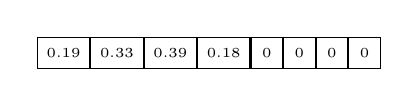
\begin{tikzpicture} [
                    cell/.style={draw, minimum width={4mm}, minimum height={4mm}, solid, thin}
                ]
                \matrix [nodes=draw]
                {
                \node [cell] {\tiny 0.19}; & \node [cell] {\tiny 0.33};   & \node [cell] {\tiny 0.39}; & \node [cell] {\tiny 0.18}; & \node[cell]  {\tiny 0};  & \node[cell]  {\tiny 0}; & \node [cell] {\tiny 0}; & \node [cell] {\tiny 0};\\
            };
                \end{tikzpicture} 
            };
        \end{tikzpicture} 
    };
    
    \draw[edge] (eventTemplates) -- (0, -8) node [midway, fill=white] {\footnotesize \textcolor{customGreen}{feature extraction}};
    

\end{tikzpicture}
   \caption{An example of encoding log sequence into two types of feature vectors: \textit{Event count vector} and \textit{TF-IDF vector}. We assume that there is $8$ event templates in the collection, thus the output vectors are also of length $8$.}
	\label{fig:feature-extraction}
	}
\end{figure}

\begin{table}
\centering
\resizebox{\textwidth}{!}{\begin{tabular}{@{}ccc@{}}
\toprule
\textbf{Matrix type} & \textbf{Row}               & \textbf{Column}                                          \\ \midrule
\textbf{\textcolor{customRed}{Event count}}    & log sequence & Frequency of event type in the log sequence              \\
\textbf{\textcolor{customRed}{TF-IDF}}         & log sequence & IDF weighted frequency of event type in the log sequence \\ \bottomrule
\end{tabular}}
\caption{A summary of feature matrix types using in our thesis.}\label{tab:embeddings-summary}
\end{table}

\subsubsection*{Event Count Matrix}
A simple approach to obtain such a representation is to create an event count vector for each log sequence. In other words, for each log sequence, we count the number of event type identifiers and store it as a row vector of an event count matrix. The length of the vector corresponds to the number of unique event types detected in the log parsing section, and each component of the vector corresponds to an event type. The value at each position in the vector is the frequency of the event types. For event types that did not occur in the log sequence, the value is zero. Thus, one row of the event count matrix represents a single log sequence. The valuable information that contributes to the machine learning model behind the event count matrix is determining what a normal number of events is and what it means to deviate from the normal counts.

%http://essay.utwente.nl/83142/1/Ma_MA_FacultyOfEEMathematicsAndCS.pdf illustration

This way of constructing the event count matrix is known in the literature as a natural language processing (NLP) model for feature extraction called \textit{Bag-of-Words} (BoW) \cite{informationRetrieval2008}. BoW treats each log sequence as a \textit{document} and for each \textit{word} (in our case, a word is an event type) in a document, a \textit{weight} is assigned. The weight depends on the number of occurrences of the term in the document. The length of the vector is equal to the number of unique words in the database (analogous to all parsed event types). The weight score is then called \textit{Term Frequency} (TF) and denoted by $tf_{t,d}$, where subscript $t$ refers to the term (event type) and $d$ refers to the document (log sequence) and $f_{t,d}$ is a frequency of term $t$ in document $d$. The term frequency describes the importance of an event type in a log sequence.

\begin{gather}
    tf_{t,d} = \dfrac{f_{t,d}}{\sum_{t'}f_{t', d}}
\end{gather}

In other words, $tf_{t, d}$ is the probability of $t$ occurring in $d$.

\subsubsection*{TF-IDF}
Another weighting scheme widely used in Information Retrieval is called \textit{term frequency–inverse document frequency} (TF-IDF). 

If we use only the standard term frequency, we have to deal with an important issue. After defining the term frequency, all event types are considered equally important \cite{informationRetrieval2008}. However, we also want to know how important a term is not only in a document, but in the whole dataset. This is where another weighting score, \textit{inverse document frequency} (IDF) comes into play. Let's first define \textit{document frequency} (DF). The document frequency $df_t$ is defined as the number of documents in the collection that contain the term $t$. Then, the inverse document frequency $df_t$ of the term $t$ is defined as: 


\begin{gather}
    idf_t = \log{\dfrac{N}{df_t}}
    \label{formula:idf}
\end{gather}

where $N$ is the total number of documents in the collection. It can be observed that if a term is rare in the collection, the $idf$ is high, and if the term is frequent, the $idf$ is low.

By definition, the TF-IDF weight of a term $t$ in document $d$ is a product of two quantities: the term frequency $tf_t$ and the inverse document frequency $idf_t$:

\begin{gather}
    tf\text{-}idf_{t, d} = tf_{t,d} \times idf_t
    \label{formula:tfidf}
\end{gather}

The intuition behind the components of TF-IDF weighting is that term frequency gives higher weight to terms that occur frequently in a single document. In contrast, the inverse document frequency gives a lower score to words that occur frequently throughout the collection, since we are more interested in those that occur infrequently. Thus, the weight $tf\text{-}idf_{t, d}$ of the term $t$ in document $d$ is 

\begin{enumerate}
    \item higher, if the term $t$ is occurs frequently in the small number of documents
    \item lower, if the term $t$ is rarely occurring in the high number of documents or if the term $t$ is rarely occurring in the document $d$
    \item lowest, if the term $t$ occurs in all documents of the collection
\end{enumerate}

As a result, the feature vector of the log sequence is a vector whose value for each dimension is defined by \ref{formula:tfidf}.

The final vectorization of the log sequence involves normalizing the IDF weight by scaling it between 0 and 1. There are several ways to normalize the IDF, but we chose the common approach of applying the \textit{logistic} (sigmoid) function to normalize IDF:

\begin{align*}
    tf\text{-}idf_{t, d} &= tf_{t,d} \times \sigma(idf_t) \\
    \sigma(x) &= \dfrac{1}{1 + e^{-x}}
\end{align*}

\subsubsection*{TF-IDF Example}
We show an example of computing TF-IDF in our case where we work with log sequences instead of documents and event type identifiers instead of terms. Suppose we have a collection of log sequences and we have $8$ event templates extracted from our dataset. Each log message found in the log sequence is identified by the corresponding event type identifier starting from $1$ to $8$, as shown in Table \ref{tab:tfidfexample1}.

\begin{table}
\centering
\begin{tabular}{@{}C{10cm}C{10cm}@{}}
\toprule
\textbf{Log sequence ID} & \textbf{Event Types} \\ \midrule
$l_1$                       & {$[1, 4, 1, 3, 7]$}               \\
$l_2$                         & {$[3, 3, 3, 8, 4]$}               \\
$l_3$                         & {$[2, 7]$}               \\
$l_4$                         & {$[3, 3, 6, 8, 4, 6]$}               \\ \bottomrule
\end{tabular}
\caption{An example of log sequences that include different sets of log messages. The log message is represented by the event type identifier.}\label{tab:tfidfexample1}
\end{table}

To compute the term frequency, we find the frequencies of the event types in each log sequence and then normalize the frequencies to sum the row vectors to $1$. Continuing with our sample set of log sequences, the TF score calculation is described in Table \ref{tab:tfidfexample2}.

\begin{table}[!h] 
\begin{subtable}[b]{1\textwidth}
\centering
  \begin{tabular}{@{}ccccccccc@{}}
        \toprule
        \backslashbox{Log sequence ID}{Event type ID} & \textbf{1} & \textbf{2} & \textbf{3} & \textbf{4} & \textbf{5} & \textbf{6} & \textbf{7} & \textbf{8} \\ \midrule
        $l_1$                     & 2          & 0          & 1          & 1          & 0          & 0          & 1          & 0          \\ \midrule
        $l_2$                     & 0          & 0          & 3          & 1          & 0          & 0          & 0          & 1          \\ \midrule
        $l_3$                     & 0          & 1          & 0          & 0          & 0          & 0          & 1          & 0          \\ \midrule
        $l_4$                     & 0          & 0          & 2          & 1          & 0          & 2          & 0          & 1          \\ \bottomrule
        \end{tabular}
        
        \caption{Computation of the frequency $f_{t,d}$ of term $t$ in document $d$.}
    \end{subtable} \\
	\hfill
	\\
    \begin{subtable}[b]{1\textwidth}
    \centering
      \resizebox{\textwidth}{!}{\begin{tabular}{@{}ccccccccc@{}}
        \toprule
        \backslashbox{Log sequence ID}{Event type ID} & \textbf{1} & \textbf{2} & \textbf{3} & \textbf{4} & \textbf{5} & \textbf{6} & \textbf{7} & \textbf{8} \\ \midrule
        $l_1$                     & 2/5          & 0          & 1/5          & 1/5          & 0          & 0          & 1/5          & 0          \\ \midrule
        $l_2$                     & 0          & 0          & 3/5          & 1/5          & 0          & 0          & 0          & 1/5          \\ \midrule
        $l_3$                    & 0          & 1/2          & 0          & 0          & 0          & 0          & 1/2          & 0          \\ \midrule
        $l_4$                     & 0          & 0          & 1/3          & 1/6          & 0          & 1/3          & 0          & 1/6          \\ \bottomrule
        \end{tabular}}
        \caption{Computation of the TF score $tf_{t,d} = \dfrac{f_{t,d}}{\sum_{t'}f_{t', d}}$.}
    \end{subtable}%
    \caption{Computation of the TF score.}
	\label{tab:tfidfexample2}
\end{table}

To compute the IDF, we first compute the document frequency $df_t$ of each term and use the formula \ref{formula:idf} to obtain the inverse document frequencies. For illustrative purposes, we omit the normalization.

\begin{table}[!h] 
\begin{subtable}[b]{1\textwidth}
\centering
  \begin{tabular}{@{}ccccccccc@{}}
        \toprule
        \backslashbox{Log sequence ID}{Event type ID} & \textbf{1} & \textbf{2} & \textbf{3} & \textbf{4} & \textbf{5} & \textbf{6} & \textbf{7} & \textbf{8} \\ \midrule
        \textbf{$l_1$}                     & 2          & 0          & 1          & 1          & 0          & 0          & 1          & 0          \\ \midrule
        \textbf{$l_2$}                     & 0          & 0          & 3          & 1          & 0          & 0          & 0          & 1          \\ \midrule
        \textbf{$l_3$}                     & 0          & 1          & 0          & 0          & 0          & 0          & 1          & 0          \\ \midrule
        \textbf{$l_4$}                     & 0          & 0          & 2          & 1          & 0          & 2          & 0          & 1 \\ \midrule
        $\mathbf{n_t}$                  & 1          & 1          & 3          & 3          & 0          & 1          & 2          & 2         
        \\ \bottomrule
        \end{tabular}
        
        \caption{Computation of the document frequency $df_{t}$ of term $t$.}
    \end{subtable} \\
	\hfill
	\\
    \begin{subtable}[b]{1\textwidth}
    \centering
      \resizebox{\textwidth}{!}{\begin{tabular}{@{}ccccccccc@{}}
        \toprule
        \backslashbox{Log sequence ID}{Event type ID} & \textbf{1} & \textbf{2} & \textbf{3} & \textbf{4} & \textbf{5} & \textbf{6} & \textbf{7} & \textbf{8} \\ \midrule
        \textbf{$l_1$}                     & 0.602          & 0,602          & 0.125          & 0.125          & 0          & 0.602          & 0.301          & 0.301         \\ \bottomrule
        \end{tabular}}
        \caption{Calculating the IDF score $idf_t = \log{\dfrac{N}{df_t}}$. In our example, $N=4$ since there are $4$ log sequences in the collection. For example, the IDF weight of event type $1$ is calculated as $idf_1 = \log{\dfrac{4}{1}} = 0,602$.}
    \end{subtable}%
    \caption{Computation of the IDF score.}
	\label{tab:tfidfexample3}
\end{table}

The final step is to calculate the product $TF \times IDF$ and the values are shown in Table \ref{tab:tfidfexample4}.

\begin{table}[!h]
    \centering
    \resizebox{\textwidth}{!}{\begin{tabular}{@{}ccccccccc@{}}
        \toprule
        \backslashbox{Log sequence ID}{Event type ID} & \textbf{1} & \textbf{2} & \textbf{3} & \textbf{4} & \textbf{5} & \textbf{6} & \textbf{7} & \textbf{8} \\ \midrule
        \textbf{$l_1$}                     & 0.2408          & 0          & 0.025          & 0.025          & 0          & 0          & 0.0602          & 0          \\ \midrule
        \textbf{$l_2$}                     & 0          & 0          & 0.075          & 0.025          & 0          & 0          & 0          & 0.0602          \\ \midrule
        \textbf{$l_3$}                     & 0          & 0.301          & 0          & 0          & 0          & 0          & 0.1501          & 0          \\ \midrule
        \textbf{$l_4$}                     & 0          & 0          & 0.042          & 0.021          & 0          & 0.201          & 0          & 0.05
        \\ \bottomrule
        \end{tabular}}
    \caption{TF and IDF scores from the example are multiplied to get TF-IDF}.
    \label{tab:tfidfexample4}
\end{table}

We assume that by using TF-IDF weighting, we obtain additional information about the event type distribution not only with respect to the log sequences, but also in the whole dataset, which could potentially increase the performance of the ML model. 

\section{Anomaly Detection}

Now that we have created the feature matrices, machine learning methods can be applied to detect outliers in the data. For our experiments, we use an open-source machine learning toolkit \textit{Loglizer}. 

\subsection{Loglizer}
\label{subscetion:loglizer}

Loglizer\footnote{https://github.com/logpai/loglizer} is an open-source machine learning based log analysis toolkit for automated anomaly detection written in Python \cite{he2016}. Loglizer was developed for automated anomaly detection as a part of LogPAI\footnote{\url{http://www.logpai.com}}, a collection of AI-based log analysis solutions. These log analysis tools have already been deployed by industrial teams at Microsoft and Huawei. It includes three supervised anomaly detection models (\textit{Logistic Regression, Decision Tree, Support Vector Machine}) and six unsupervised anomaly detection models (\textit{Local Outlier Factor, One-Class SVM, Isolation Forest, Principal Component Analysis, Invariants Mining, Clustering}). At the time of writing, two more unsupervised models were under development (\textit{DeepLog, AutoEncoder}). 

We chose to use a third-party toolkit for several reasons. First, since the algorithms we use in our experiments are already implemented, there is no need to completely reinvent the wheel and write the implementation ourselves. This way, we can avoid a time-consuming process and instead focus on the main purpose of our research - to investigate whether applying different anomaly detection techniques to a real-world dataset can lead to successful results and how to approach it.

Another advantage is that the Loglizer anomaly detectors work with log sequences. This means that each of the models is trained on a set of log sequences, and the output of the detector classifies whether a single log sequence is an anomaly or not. As described in Section~\ref{section:featureEngineering}, we use windowing to generate the log sequences, making the Loglizer toolkit an excellent fit for our research context. Specifically, four methods were used in our research: Invariants Mining, Isolation Forest, and PCA . The underlying algorithms behind these tools are presented in Section \ref{section:anomalyDetectionLiteratureReview}.

The implemented anomaly detection methods are evaluated on a public dataset, HDFS. The logs in the HDFS dataset were collected from the Amazon EC2 platform and contain $11\,175\,629$ entries \cite{xu2009}. Loglizer provides benchmarking results for both supervised and unsupervised methods separately using this dataset, which can be found in Table \ref{table:loglizer}. The evaluation metrics are explained in Section \ref{section:evaluationMetrics}. Benchmarking gives a better idea of the expected performance of the anomaly detection methods we intend to use in our work.  

Last but not least, Loglizer makes it easier to reproduce, understand and customize the experiments since the code is open source.

\begin{table}[h]
\centering
\begin{tabular}{@{}cccc@{}}
\toprule
\multicolumn{4}{c}{\textbf{HDFS}} \\ 
\textbf{Model}    & \textbf{Precision} & \textbf{Recall} & \textbf{F1} \\  \toprule \midrule
\multicolumn{4}{c}{\textit{Supervised Methods}}                        \\ \midrule
LR                & 0.955              & 0.911           & 0.933       \\
Decision Tree     & 0.998              & 0.998           & 0.998       \\
SVM               & 0.959              & 0.970           & 0.965       \\ \midrule
\multicolumn{4}{c}{\textit{Unsupervised Methods}}                      \\ \midrule
LOF      & 0.967              & 0.561           & 0.710       \\
One-Class SVM     & 0.995              & 0.222           & 0.363       \\
Isolation Forest  & 0.830              & 0.776           & 0.802       \\
PCA               & 0.975              & 0.635           & 0.769       \\
Invariants Mining & 0.888              & 0.945           & 0.915       \\
Clustering        & 1.000              & 0.720           & 0.837       \\ \bottomrule
\end{tabular}
\caption{Benchmarking results of three supervised and six unsupervised anomaly detection methods on HDFS dataset \cite{he2016}}.
\label{table:loglizer}
\end{table}

\subsection{Experiment Workflow}
Running machine learning experiments is typically an iterative process, with each iteration requiring different configuration parameters, input training and testing datasets, and a lot of file processing. The same is true for our anomaly detection experiments. We obtained several raw datasets from the SmartConnect system. We selected four anomaly detection methods, with each method requiring a different dataset as well as its own parameter configuration. Each raw dataset must be parsed from its original JSON file into a unified structure, cleaned up, and erroneous log entries removed. Then, a log parser program is applied to obtain an event type identifier for each log message. Finally, we use two different feature matrix representations as input to anomaly detection methods. After we obtain trained models for each dataset, the evaluation follows. With so many dependent processes that need to be performed for each iteration of the experiment, where things can very easily become messy, it is desirable to have an automated workflow system. Although our work is not a software engineering thesis and thus the focus was not on a perfectly extensible workflow, we tried to find a solution that would save the time required to run experiments.

We created a Makefile-based pipeline containing a set of Python scripts to facilitate experiments. The goal was to have a reproducible, modular, and scalable solution to deal with the complexity of running experiments. In this section, we will briefly describe the architecture of this pipeline and the implementation of the experiment scripts.
 
 \subsubsection*{Makefile}
The execution of experiments is orchestrated by the GNU \textit{make} instructions described in the Makefile scripts. A Makefile consists of a set of rules that generate target files when one of their dependencies changes. We chose Makefile because it directly enforces a modular character to our workflow. Every rule must follow the shape:

\begin{verbatim}
    target ... : prerequisities ... 
        recipe
        ...
\end{verbatim}

Normally, targets and prerequisites are filenames and recipes are commands. A Makefile can be expressed by a directed acyclic dependency graph \cite{feldman1979make}. The dependency graph of our Makefile is shown in Figure \ref{fig:makefile}. 
 
 Each target contained in the Makefile operates on the \texttt{DATASET} variable assignment.  \texttt{DATASET} represents the name of the dataset that must exist in the \texttt{data/raw/} directory of the project folder before any of the targets are executed, so we call it a \textit{prerequisity} or a \textit{dependency}. The variable can be set from outside the Makefile as part of the command line. Changing the value of \texttt{DATASET} directly affects the names of the generated output files. By running \texttt{make} in the directory containing the Makefile and assigning \texttt{DATASET} variable, we can manage the workflow of the experiment:
 
 \begin{itemize}
     \item \texttt{make} \textit{data} \texttt{DATASET=<dataset name>}
     \begin{itemize}
         \item Parses JSON file with raw data into a panda's DataFrame
         \item Flattens columns of the DataFrame that contain nested JSON structures
         \item Executes log abstraction by processing log messages, extracting an event type for each log message and appending event type column to the DataFrame
         \item Stores DataFrame with preprocessed logs 
         \item Extracts event count and TF-IDF feature matrices
         \item Stores feature matrices
     \end{itemize}
     \item \texttt{make} \textit{train} \texttt{DATASET=<dataset name>}
     \begin{itemize}
         \item Executes training script and generates invariant mining, isolation forest, log clustering and PCA models using event count and TF-IDF feature matrices
         \item Stores models
     \end{itemize}
     \item \texttt{make} \textit{evaluate} \texttt{DATASET=<dataset name>}
     \begin{itemize}
         \item Executes evaluation script for invariant mining, isolation forest, log clustering and PCA models trained using event count and TF-IDF feature matrices by detecting anomalies on provided labeled dataset
         \item Generates precision, recall and F1 score into CSV files stored in \texttt{\justify results/metrics} directory
         \item Generates labels predicted by all the models into CSV files stored in~\texttt{results/predictions} directory
     \end{itemize}
     \item \texttt{make} \textit{all} 
     \begin{itemize}
         \item Runs all modules of the workflow
     \end{itemize}
     \item \texttt{make} \textit{clean} \texttt{DATASET=<dataset name>}
     \begin{itemize}
         \item Cleans up all generated files related to \texttt{DATASET} including the trained model, if it exists
     \end{itemize}
 \end{itemize}
 
 \begin{figure}[!h] \centering {
   \begin{tikzpicture} [
    edge/.style={-latex,shorten >=1pt, thin, color=customGrey},
    line/.style={-,shorten >=1pt, thin, color=customGrey},
    fileTarget/.style={rectangle, draw=customBlue, align=left, minimum width=55mm, minimum height=7mm},
    phonyTarget/.style={rectangle, draw=customRed, align=left, minimum width=20mm, minimum height=7mm}
]

\node[fileTarget, align=center] (root) at (0, 0) {\tiny data/raw/\$(DATASET).json};

\node[fileTarget, align=center] (preprocessed_tf) at (-3, -1.5) {\tiny data/preprocessed/tf/\%-preprocessed.pickle};

\node[fileTarget, align=center] (preprocessed_tfidf) at (3, -1.5) {\tiny data/preprocessed/tfidf/\%-preprocessed.pickle};

\draw[edge] (root) -- (preprocessed_tf);
\draw[edge] (root) -- (preprocessed_tfidf);

\node[fileTarget, align=center] (features_tf) at (-3, -3) {\tiny data/features/tf/\%.npy};

\node[fileTarget, align=center] (features_tfidf) at (3, -3) {\tiny data/features/tfidf/\%.npy};

\draw[edge] (preprocessed_tf) -- (features_tf);
\draw[edge] (preprocessed_tfidf) -- (features_tfidf);

\node[phonyTarget, align=center] (data) at (0, -4.5) {\tiny data};

\draw[edge] (features_tf) -- (data);
\draw[edge] (features_tfidf) -- (data);

\node[fileTarget, align=center] (model_tf) at (-3, -6) {\tiny models/tf/\%.model};

\node[fileTarget, align=center] (model_tfidf) at (3, -6) {\tiny models/tfidf/\%.model};

\draw[edge] (features_tf) -- (model_tf);
\draw[edge] (features_tfidf) -- (model_tfidf);

\node[phonyTarget, align=center] (train) at (0, -7.5) {\tiny train};

\draw[edge] (model_tf) -- (train);
\draw[edge] (model_tfidf) -- (train);

\node[fileTarget, align=center] (results) at (0, -9) {\tiny results/\%.csv};

\draw[edge] (model_tf) -- (results);
\draw[edge] (model_tfidf) -- (results);

\node[phonyTarget, align=center] (evaluate) at (0, -10.5) {\tiny evaluate};

\draw[edge] (results) -- (evaluate);

\node[phonyTarget, align=center] (all) at (0, -12) {\tiny all};

\draw[edge] (evaluate) -- (all);

\end{tikzpicture}
   \caption{A dependency graph for a Makefile to perform experiments in our thesis. Blue rectangles represent \textit{file targets} and red rectangles represent \textit{phony targets}. Phony targets are targets that do not create or update a file, but instead represent a name for a sequence of commands to execute. Phony targets enable the modular execution of our experiments.}
	\label{fig:makefile}
	}
\end{figure}

Models and their configurations that are trained in the pipeline can be specified within the Makefile.

\subsubsection*{Scripts Implementation}
 A consistent file naming convention and file organization in directories and subdirectories is critical for automated experiments. For an example of the directory structure of our experiments designed for use with Makefile, see the Appendix \ref{appendix:dir_structure}.
 
 Each machine learning method has three Python scripts in the \texttt{src/models} directory: \textit{train}, \textit{evaluate}, and the \textit{model} itself. 
 
 Each \textit{model} script acts as a wrapper with a common interface that contains an algorithm-providing library (in our case, we use the LogLizer library, as described in Section \ref{subscetion:loglizer}) and allows calling the following methods:
 
\begin{itemize}
    \item \texttt{\_\_init\_\_}
    \item \texttt{fit}
    \item \texttt{predict}
    \item \texttt{evaluate}
    \item \texttt{save}
    \item \texttt{load}
\end{itemize}

The advantage of having a wrapper on top of the actual model is that it can easily be replaced by another library that provides the model implementation, or we can provide our own implementation.

As you can see from the list above, each model also contains \texttt{save} and \texttt{load} methods. They are included in the model as a means of serializing and deserializing the trained model. The reason for this is that training a model is usually a very time-consuming task. The ability to load an already trained model saves us the trouble of training the model every time it is needed. A serialized model can be conveniently restored later and used for evaluation or prediction. We use the library \texttt{pickle}\footnote{https://docs.python.org/3/library/pickle.html}, which converts any Python object into a byte stream. The process of serializing the data is then called "pickling" and the deserialization is called "unpickling".

\textit{Train} scripts allow optional and model-specific parameters to tune the models. These parameters can be modified in the Makefile. Then, the preprocessed data is simply loaded, the model is instantiated, and the model training process is executed. Finally, the trained model is stored in a pickle. 
 
\textit{Evaluate} scripts include loading the trained model and executing the \texttt{\justify evaluate} method to obtain metrics and predictions.

As shown in the directory structure in the Appendix \ref{appendix:dir_structure}, preprocessed features, trained models, and resulting metrics and predictions are stored in either the \texttt{tf} or \texttt{tfidf} folder, depending on which feature extraction method the particular file belongs to. \texttt{tf}, as an abbreviation for term frequency, is an equivalent to what we call \texttt{event count} in our work, as we explained in detail in Section \ref{subsection:features}. For brevity, we use \texttt{tf} in our file structure.

\subsection{Mapping from Prediction Back to Log Entry}
\label{methodology:mapping-predictions-back}
Once the output is computed, we get a prediction for each window of the input dataset. This is true regardless of the specific machine learning model used for the computation. 
This type of output, which consists of ones and zeros, is not very helpful if we want to understand why we got these results and whether they are correct. Ideally, we would want more detailed information about each window.
Typically, the windows that are identified as anomalous would be of interest, as they are expected to be less frequent and more important. However, there are use cases where we want to examine all windows, especially in the debugging phase. 

From a feature vector of a given window, only the ID and the frequency of the event type are given, the template and the order are lost.
After discussing with domain experts what would be valuable information about a time window, we concluded that it should be included with every window:
\begin{itemize}
    \item \textit{How frequent is each of the event types and what is the template for each event.}\\
    We create a histogram, ordered in descending order from the most frequent events to the least frequent. This gives a good overview of what the state of the system is in a given time window. 
    \item \textit{Raw trace of logs within the window.}\\
    The histogram is a good place to start, but in some cases the detail and preserved order matters. In some cases, we also need to know the variable parts of the log messages that are missing from the log templates to get a clear picture of what was going on in the system. Therefore, we also order the traces of the raw logs according to the time in which they occurred.
    \item \textit{What time range a window corresponds to.}\\
    It is easy to map from a window index to a human readable time. This way, an expert can tell if something special happened in the system. For example, regular tests may occur daily at certain times, which may explain some behaviour.
\end{itemize}
 
% Flowchart: https://bost.ocks.org/mike/make/

